%В работах \cite{Thompson,Tong} описан устойчивый итерационный алгоритм эволюции поверхностной сетки, сохраняющий целевой объем льда.
The articles \cite{Thompson,Tong} describe a stable iterative grid evolution algorithm that preserves the target volume of ice.
%В нем используется ряд улучшений по сравнению с классическими методами.
It uses several improvements over the classical methods.

%Многослойный подход, реализованный в этом методе, не использует константное количество шагов - величина наращиваемого объема на каждом шаге алгоритма рассчитывается исходя из максимально допустимой доли временного шага обледенения, после превышения которого возможно развитие численной нестабильности в эволюции поверхности.
The multilayer approach implemented in this method does not use a constant number of steps - the value of the increased volume at each step of the algorithm is calculated based on the maximum allowable fraction of the icing time step, after exceeding which numerical instability may occur in the evolution of the surface.
%Наиболее очевидный случай возникает, когда проекции нормалей граней пересекаются, в этом случае слишком большой временной шаг приведет к складыванию поверхности.
The most obvious case occurs when the face normal projections intersect, in which case too large a time step will cause the surface to fold.
%Чтобы идентифицировать грани, которые будут демонстрировать подобное поведение на текущем временном шаге, предполагается, что объем, образованный путем вытягивания треугольной грани с использованием параллельной плоскости смещения, образует призматоид, объем которого определяется кубической функцией высоты $h$:
In order to identify faces that will exhibit such behavior at the current time step, it is assumed that the volume formed by extruding a triangular face using a parallel displacement plane forms a prismatoid whose volume is given by the cubic function of the height $h$:

\begin{equation}\label{Tong:1}
V(h)=ah+bh^2+ch^3
\end{equation}

%где константы $a$, $b$, $c$ определяются позициями узлов грани, их нормалей и нормалью грани.
where the constants $a$, $b$, $c$ are determined by the positions of the face nodes, their normals, and the face normal.
%Рассмотрим корни квадратного уравнения, которое получается в результате дифференцирования уравнения \ref{Tong:1}.
Consider the roots of the quadratic equation, which is obtained as a result of differentiation of the equation \ref{Tong:1}.
%Если корни являются положительными вещественными значениями, наименьший положительный корень определяет высоту, на которой достигается максимальный объем, которая обозначается как $V_{max}$, иначе функция монотонна с возрастанием и ограничение на шаг в данной грани не требуется.
If the roots are positive real values, the smallest positive root determines the height at which the maximum volume is reached, which is denoted as $V_{max}$, otherwise the function is monotonic with increasing and no step restriction is required in this face.
%Исходя из этого, можно вычислить максимальную долю временного шага обледенения, которая требуется для обеспечения разумного поведения накопления объема.
From this, it is possible to calculate the maximum fraction of the icing time step that is required to ensure reasonable volume accumulation behavior.
%В дополнение к этому пределу размера шага был введен предел стабильности $\alpha_{jiao}$, который основан на том, как изменяются направления нормалей по мере эволюции поверхности \cite{Jiao}.
In addition to this step size limit, a $\alpha_{jiao}$ stability limit has been introduced, which is based on how normal directions change as the surface evolves \cite{Jiao}.
%Тогда, допустимая доля временного шага для $i$-й грани определяется как
Then, the allowable fraction of the time step for the $i$-th face is defined as

\begin{equation}\label{Tong:2}
\alpha_{\Delta t}^i=
\begin{cases}
min(s_{\Delta t}\frac{V_{max}^i}{V_f},\alpha_{jiao},1), \text{if $V_{max}^i$ exists}, \\
\alpha_{jiao}, \text{if $V_{max}^i$ doesn't exist}
\end{cases}
\end{equation}

%где $s_{\Delta t}$ ($0 < s_{\Delta t} < 1$) -- эмпирически определяемый коэффициент, $V_f$ -- текущий оставшийся объем приращения льда для $i$-й грани.
where $s_{\Delta t}$ ($0 < s_{\Delta t} < 1$) is an empirically determined coefficient, $V_f$ is the current remaining ice increment volume for the $i$-th face.
%Тогда объем, наращенный для текущего шага, равен $\alpha_{\Delta t} V_f$, где $\alpha_{\Delta t}$ представляет собой глобальное минимальное значение для всех граней.
Then the volume built up for the current step is $\alpha_{\Delta t} V_f$, where $\alpha_{\Delta t}$ is the global minimum value for all faces.

%Другой важной особенностью алгоритма является введение первичного и нулевого простанств, описанных в \cite{Jiao_null_space_smooth}.
Another important feature of the algorithm is the introduction of primary and null spaces, described in \cite{Jiao_null_space_smooth}.
%Если эволюционное движение узлов сетки происходит в первичном пространстве, то их перемещение в нулевом пространстве будет сохранять потенциальную точность второго порядка триангуляции поверхности, благодаря чему мы можем  проводить сглаживание поверхности сетки с сохранением объема.
If the evolutionary movement of mesh nodes occurs in primary space, then their movement in zero space will preserve the potential accuracy of the second order of triangulation of the surface, so that we can maintain volume when smoothing the mesh surface.
%В алгоритме используется несколько видов сглаживаний.
The algorithm uses several types of smoothing.

%Первое сглаживание -- сглаживание нормалей в вершинах и ячейках сетки.
The first smoothing is the smoothing of the normals in the mesh nodes and faces.
%Чтобы сделать возможным сглаживание в нулевом пространстве, все нормали в узлах рассчитываются так, чтобы они лежали в первичном пространстве, а перемещение узлов при наращивании льда происходит только по их нормалям.
To make smoothing possible in zero space, all normals at nodes are calculated so that they lie in primary space, and the movement of nodes during ice buildup occurs only along their normals.
%По мере эволюции, на поверхности может усиливаться шум -- если его не контролировать, может возникнуть ситуация, когда двугранный угол между гранями станет слишком малым и ограничит максимальную долю временного шага обледенения.
As evolution progresses, surface noise can increase - if left unchecked, a situation can arise where the dihedral angle between the faces becomes too small and limits the maximum fraction of the icing time step.
%Для уменьшения поверхностного шума, перед наращиванием льда применяется локальное сглаживание, регулирующее направление смещения узла в проблемных областях, чтобы оно более точно совпадало с направлениями его соседей.
To reduce surface noise, local smoothing is applied before ice builds up, adjusting the direction of node displacement in problem areas so that it more closely matches the directions of its neighbors.
%Этот метод может улучшить гладкость поверхности в некоторых ситуациях.
This method can improve surface smoothness in some situations.
%Основная цель сглаживания нормалей -— вытолкнуть точки из вогнутых областей, где нормали могут локально сходиться.
The main purpose of normal smoothing is to push points out of concave areas where normals can converge locally.
%Сглаживание нормалей достигается с помощью серий взвешенных средних, которые предназначены для придания веса нормалям, генерируемым проблемными областями.
Normal smoothing is achieved using a series of weighted averages, which are designed to give weight to the normals generated by problem areas.

%Второе сглаживание -- сглаживание высот.
The second smoothing is height smoothing.
%После вычисления доли временного шага и объема, наращиваемого для текущего шага, для эволюции поверхности необходимо определить поле высот, которое будет соответствовать этому объему, чтобы по нему определить смещения узлов сетки.
After calculating the fraction of the time step and the volume that is increased for the current step, it is necessary to determine the height field for the evolution of the surface , which will correspond to this volume, in order to determine the offsets of the grid nodes from it.
%Решение $V(h_i) = \alpha_{\Delta t} V_f$ обеспечивает поле начальных высот, которое используется для движения поверхности.
The solution $V(h_i) = \alpha_{\Delta t} V_f$ provides the initial height field that is used to move the surface.
%Цель дополнительного шага сглаживания высоты состоит в том, чтобы отфильтровать высокочастотный шум в поле высот за счет уменьшения разницы высот между соседними гранями.
The purpose of the additional height smoothing step is to filter out high-frequency noise in the height field by reducing the difference in height between adjacent faces.
%Как правило, высоты двух треугольных граней, имеющих общее ребро, не будут равными.
Usually, the heights of two triangular faces that share a common edge will not be equal.
%На данном шаге используется сглаживание высот с сохранением объема путем его перераспределения между соседними гранями.
At this step, smoothing of heights is used while preserving the volume by redistributing it between adjacent faces.

\begin{figure}
  \centering
  \begin{minipage}[h]{0.49\textwidth}
    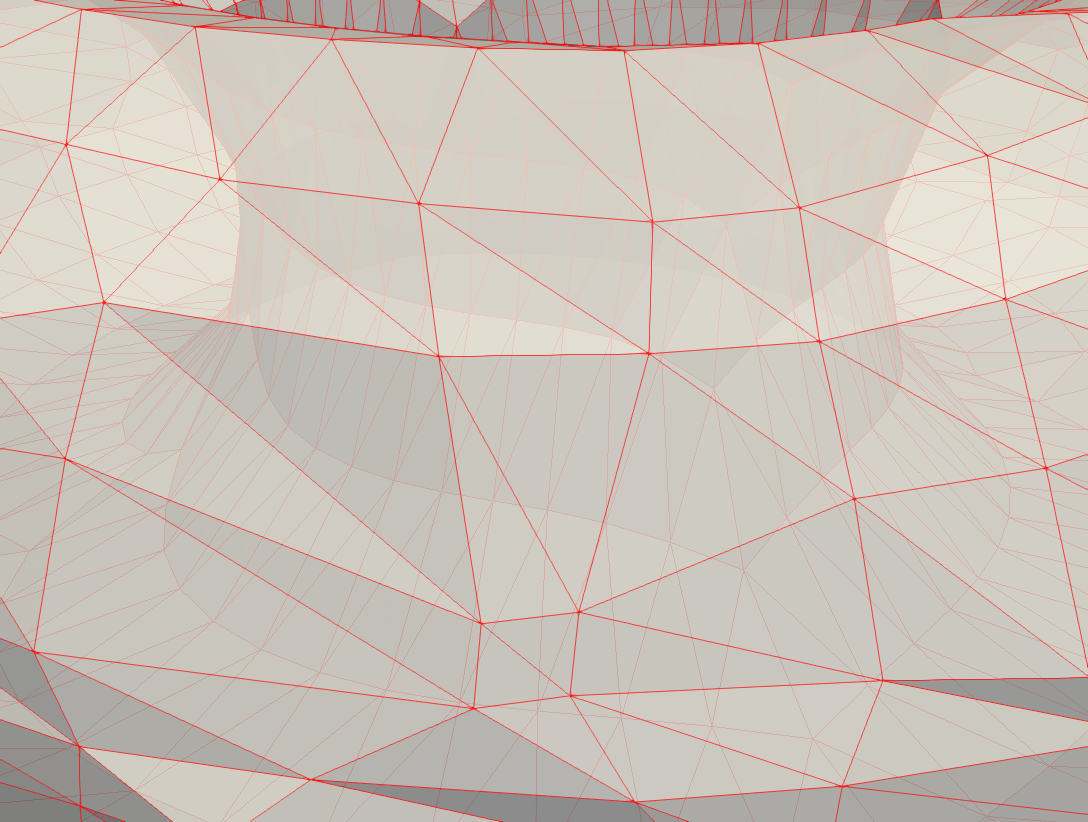
\includegraphics[width=\textwidth]{pics/pic_smooth_before.png}
    \caption{Mesh before null-space smoothing}\label{fig:pic_smooth_before}
  \end{minipage}
  \hfill
  \begin{minipage}[h]{0.49\textwidth}
    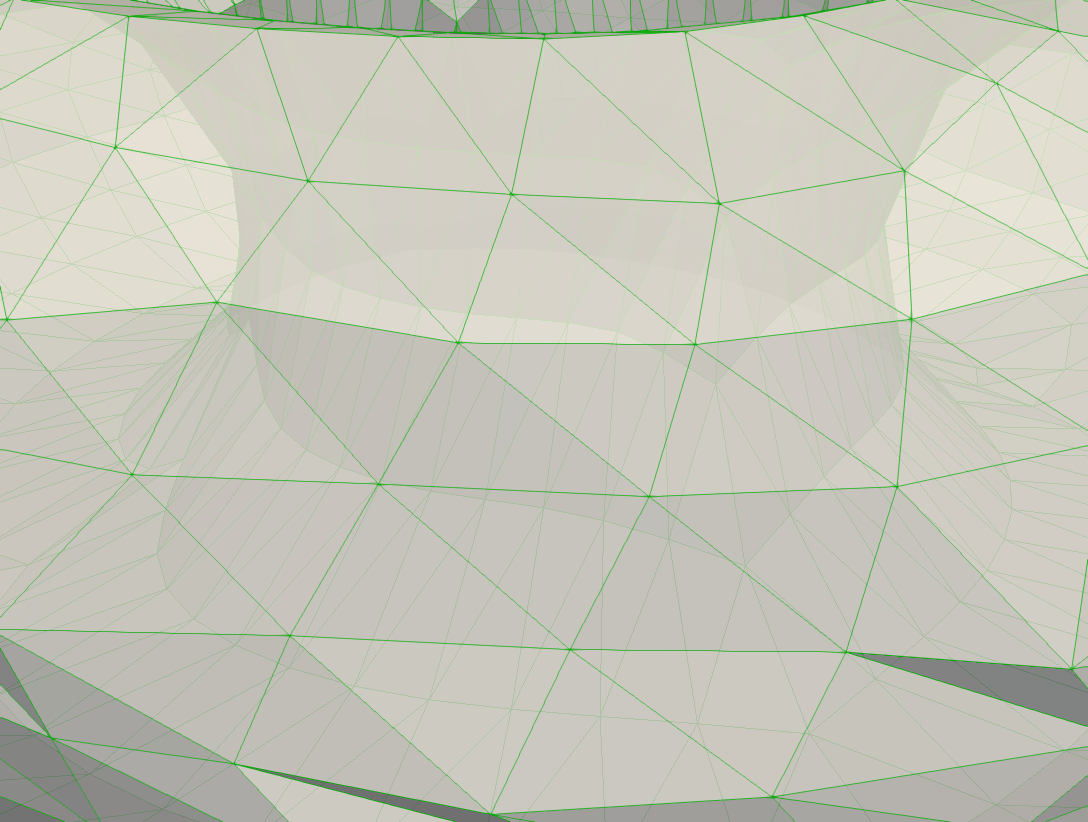
\includegraphics[width=\textwidth]{pics/pic_smooth_after.png}
    \caption{Mesh after null-space smoothing.}\label{fig:pic_smooth_after}
  \end{minipage}
\end{figure}

%Последним типом сглаживания является сглаживание в нулевом пространстве.
The last type of smoothing is null space smoothing.
%Эволюция поверхности будет стремиться упаковать узлы в вогнутые области, где сходятся нормали к поверхности, тогда как расширение сетки происходит в выпуклых областях, где нормали к поверхности расходятся.
Surface evolution will tend to pack nodes into concave regions where surface normals converge, while mesh expansion occurs in convex regions where surface normals diverge.
%Если узлы не будут перераспределены, может стать невозможным продолжать продуктивный, стабильный временной шаг.
If the nodes are not reallocated, it may become impossible to continue with a productive and stable time step.
%Для улучшения качества поверхностной сетки узлы перераспределяются на поверхности с помощью сглаживания в нулевом пространстве.
To improve the quality of the surface mesh, the nodes are redistributed on the surface using null space smoothing.
%Этот метод способен перераспределять точки, сохраняя при этом целостность базовой геометрии.
This method is able to redistribute points while maintaining the integrity of the base geometry.
%Нулевое пространство определяется касательной плоскостью (для гладких областей), касательной линией (для складок поверхности) или пустым пространством (для углов), движущиеся в нем узлы остаются на поверхности, так что объем и форма поверхности могут быть сохранены (Fig.~\ref{fig:pic_smooth_before}, Fig.~\ref{fig:pic_smooth_after}).
Null space is defined by a tangent plane (for smooth areas), a tangent line (for surface wrinkles), or empty space (for corners), nodes moving in it remain on the surface, so that the volume and shape of the surface can be preserved (Fig.~\ref{fig:pic_smooth_before}, Fig.~\ref{fig:pic_smooth_after}).